% !TEX root = ../../main.tex

\subsubsection{MIL-100(Fe)}

The enthalpy profiles on the MIL-100(Fe) powder are less homogenous
than the ones on UiO-66(Zr). Some effects can be seen with probes which
can interact with the partially reduced \ce{Fe(II)} atom, such as
carbon monoxide and propylene (\autoref{shaping:fgr:mil100isotherms}).
Indeed, when comparing both the initial Henry constants and
enthalpy of adsorption, for \ce{CO} and \ce{C3H6}, these are
higher than the values obtained on UiO-66(Zr).
With initial enthalpy of adsorption for \ce{CO} of around
\SI{45}{\kilo\joule\per\mol}, the value falls into the range of
previous~\cite{yoonControlledReducibilityMetalOrganic2010}
results for interactions with such \ce{Fe(II)} CUS.

\begin{figure}[htb]
	\centering
	\begin{subfigure}{0.45\textwidth}
		\includegraphics[width=\linewidth]{calo/MIL-100(Fe)/c3h6-mass-basis-iso}
		\caption{}%
		\label{shaping:fgr:mil100c3h6adsmol}
	\end{subfigure}%
	\begin{subfigure}{0.45\textwidth}
		\includegraphics[width=\linewidth]{calo/MIL-100(Fe)/c3h6-volume-basis-iso}
		\caption{}%
		\label{shaping:fgr:mil100c3h6adsvol}
	\end{subfigure}%
	\caption{Propylene isotherms on MIL-100(Fe) on a (a) mass
		and (b) volume adsorbent basis.}%
	\label{shaping:fgr:mil100isotherms}
\end{figure}

Comparing the powder and shaped variants, there are no
apparent differences between the two. The only discrepancy,
which can be seen on the nitrogen initial \(K_H\) follows
as a result of an ill-fitting virial parameter,
and can be assumed an error after observing the isotherm
overlap directly. It could be theorised that by activation at
a higher temperature (\SI{250}{\degreeCelsius}),
the percentage of iron trimers which would undergo reduction will
increase and a further interaction could be observed.
However, the activation temperature was chosen to allow
comparisons with the PVA study~\cite{chanutObservingEffectsShaping2016},
where temperatures over \SI{180}{\degreeCelsius} would lead to the
burn-off of the polymer binder.

The maximum loading differences (\autoref{shaping:fgr:analysismil100basis})
of MIL-100(Fe) show a very similar behaviour.
On all probes tested, a fixed capacity
loss of between 10-20\% can be seen on a mass
basis. However, the increase in density afforded by the
compression during pelletisation leads to a compensation in
performance as can be seen directly when looking at isotherms on mass and
volume material basis in \autoref{shaping:fgr:mil100c3h6adsmol} and
\autoref{shaping:fgr:mil100c3h6adsvol} respectively.

We can conclude that MIL-100(Fe) is almost unaffected by alumina shaping.
A slight loss in maximum capacity on a mass basis is compensated by a pronounced densification, which is desirable in an industrial setting.

\begin{figure}
	\centering
	\begin{subfigure}{\linewidth}
		\parbox[c]{0.1\linewidth}{\caption{}%
			\label{shaping:fgr:analysismil100henry}}%
		\parbox[b]{0.8\linewidth}{%
			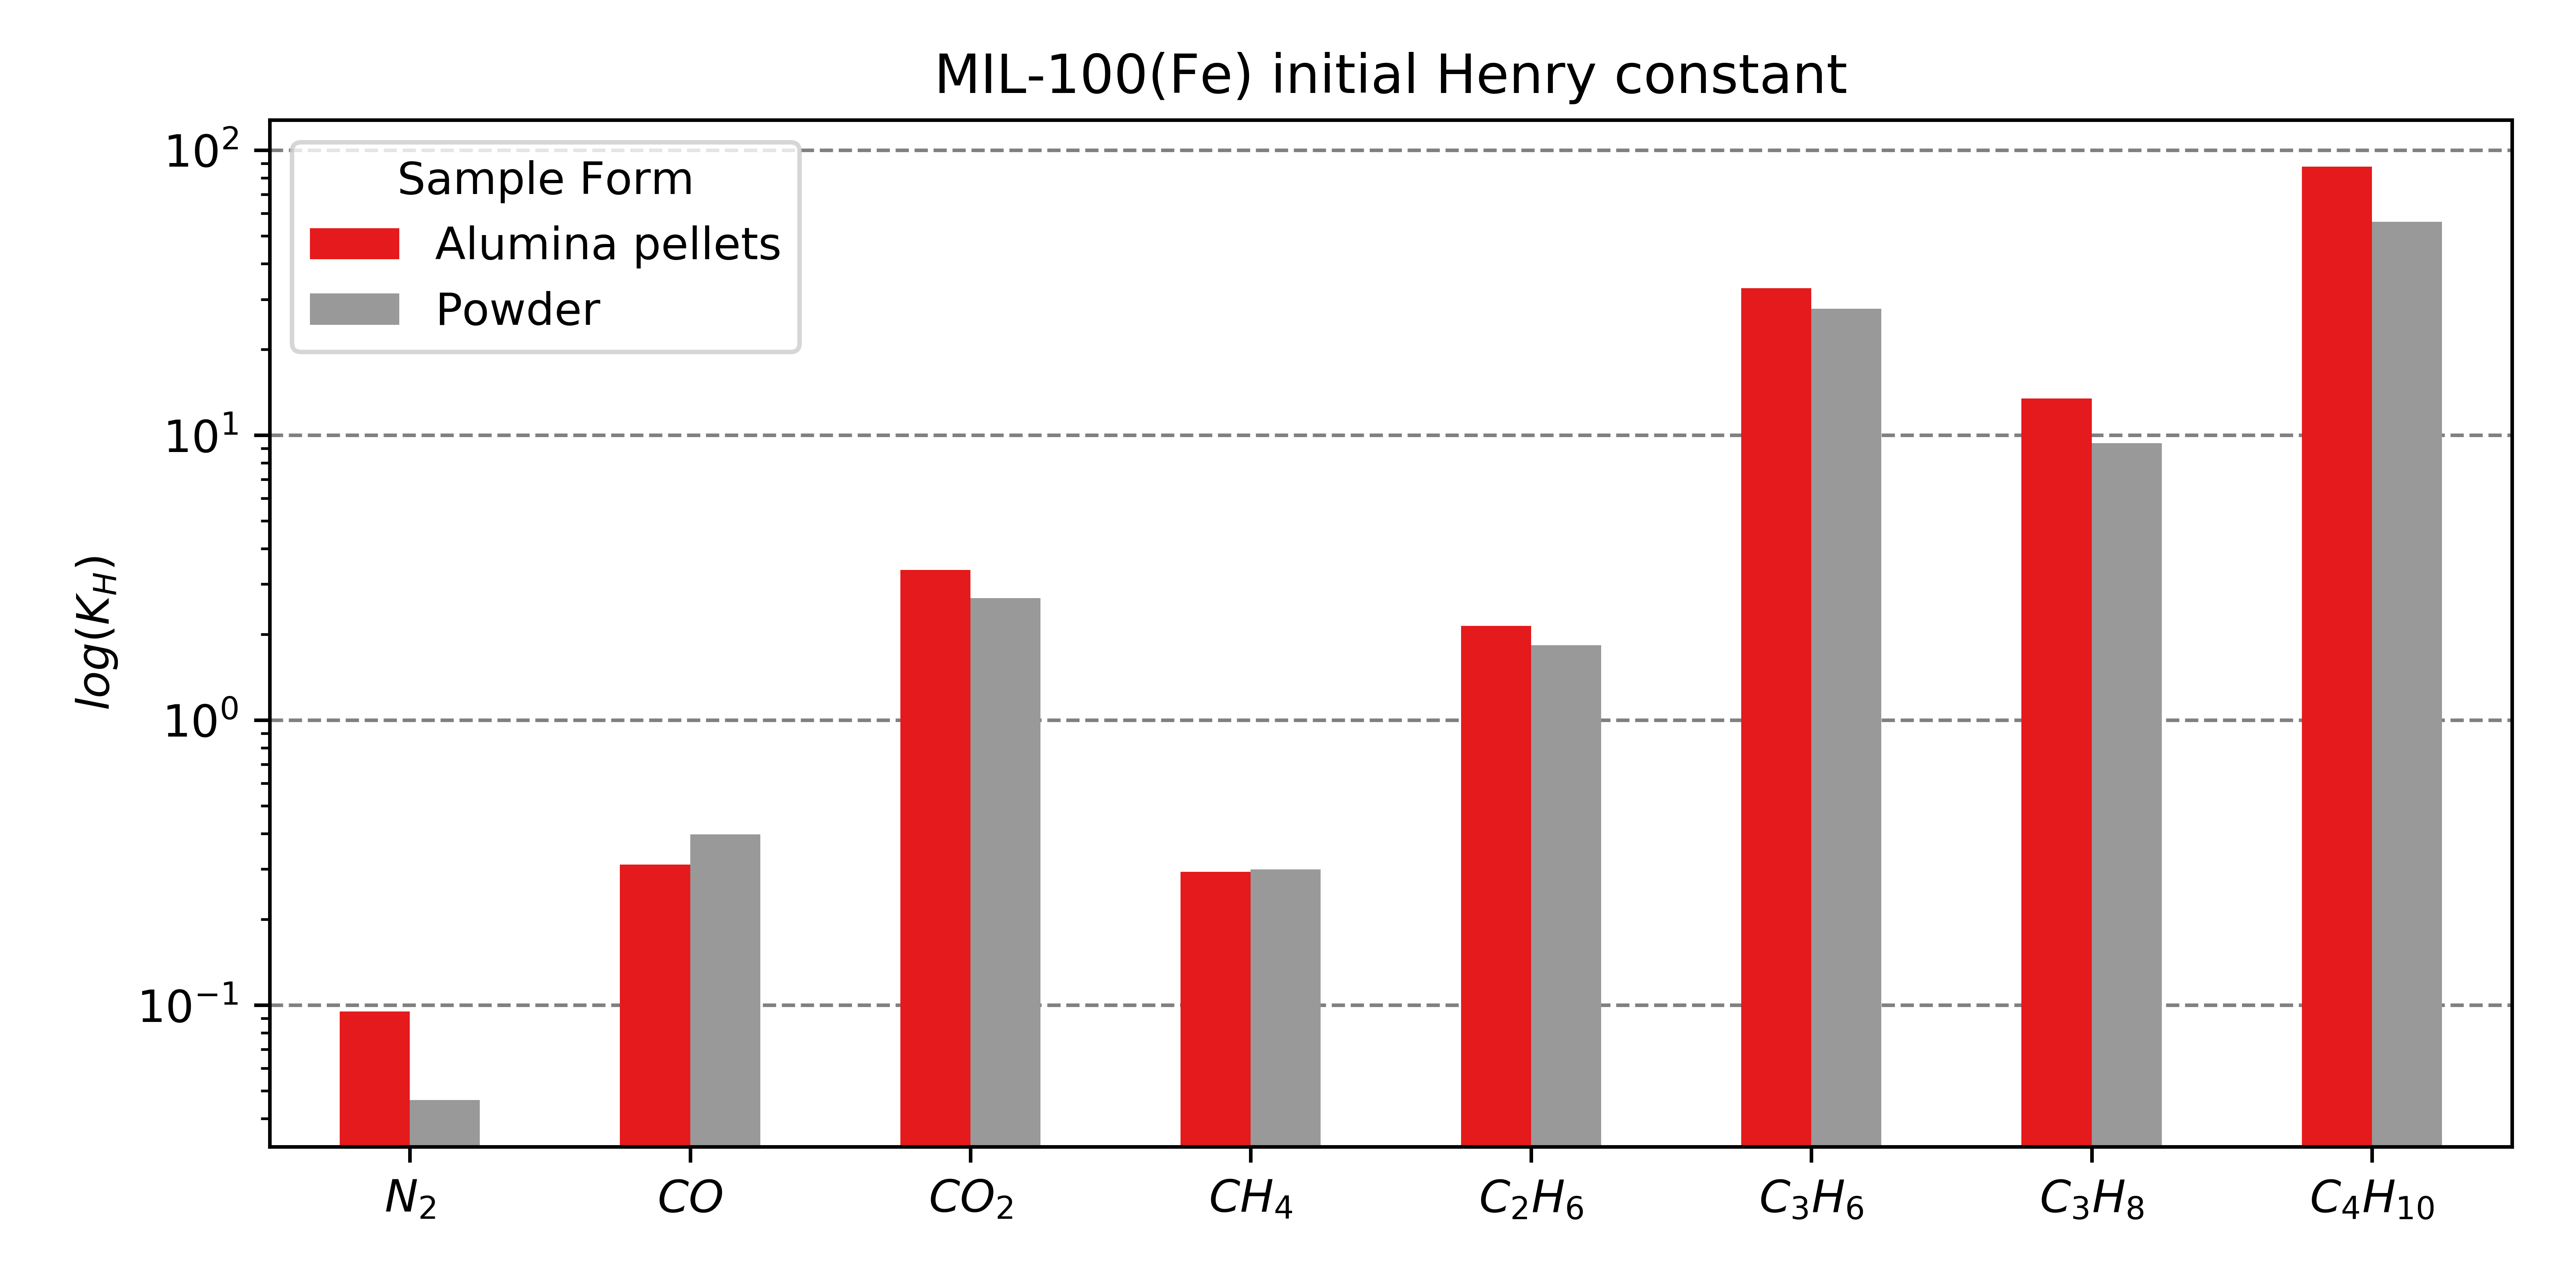
\includegraphics[width=\linewidth]{MIL-100(Fe)-henry-distribution}%
		}%
	\end{subfigure}%

	\begin{subfigure}{\linewidth}
		\parbox[c]{0.1\linewidth}{\caption{}%
			\label{shaping:fgr:analysismil100enth}}%
		\parbox[b]{0.8\linewidth}{%
			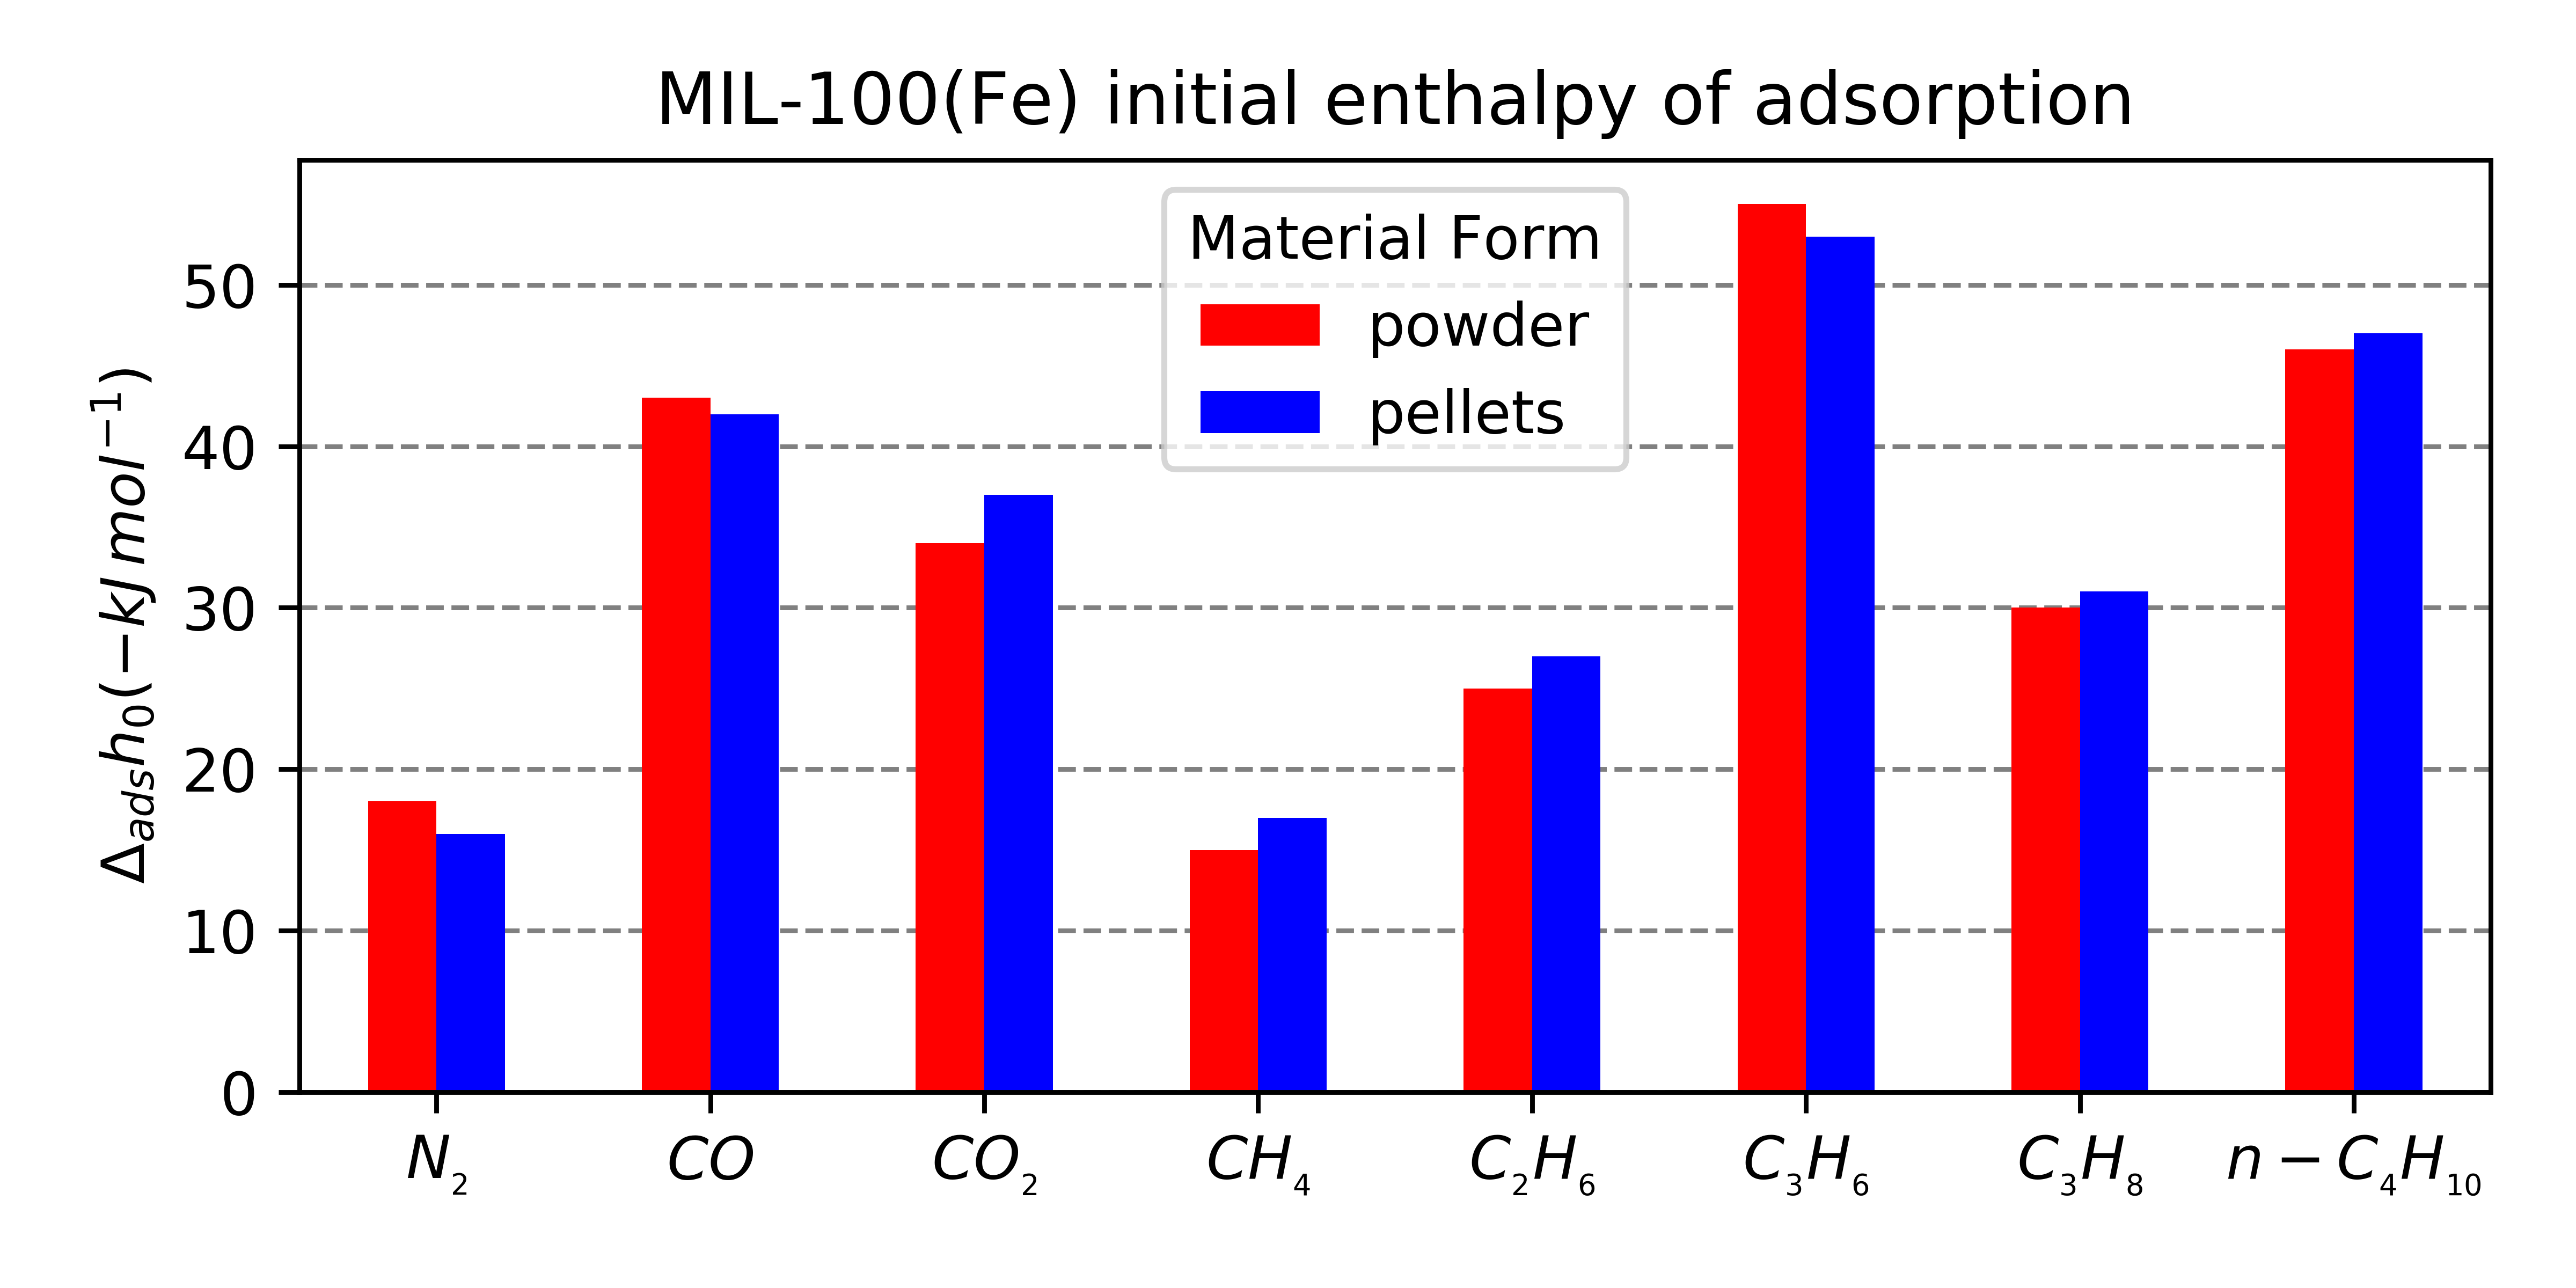
\includegraphics[width=\linewidth]{MIL-100(Fe)-enthalpy-distribution}%
		}%
	\end{subfigure}%

	\begin{subfigure}{\linewidth}
		\parbox[c]{0.1\linewidth}{\caption{}%
			\label{shaping:fgr:analysismil100basis}}%
		\parbox[b]{0.8\linewidth}{%
			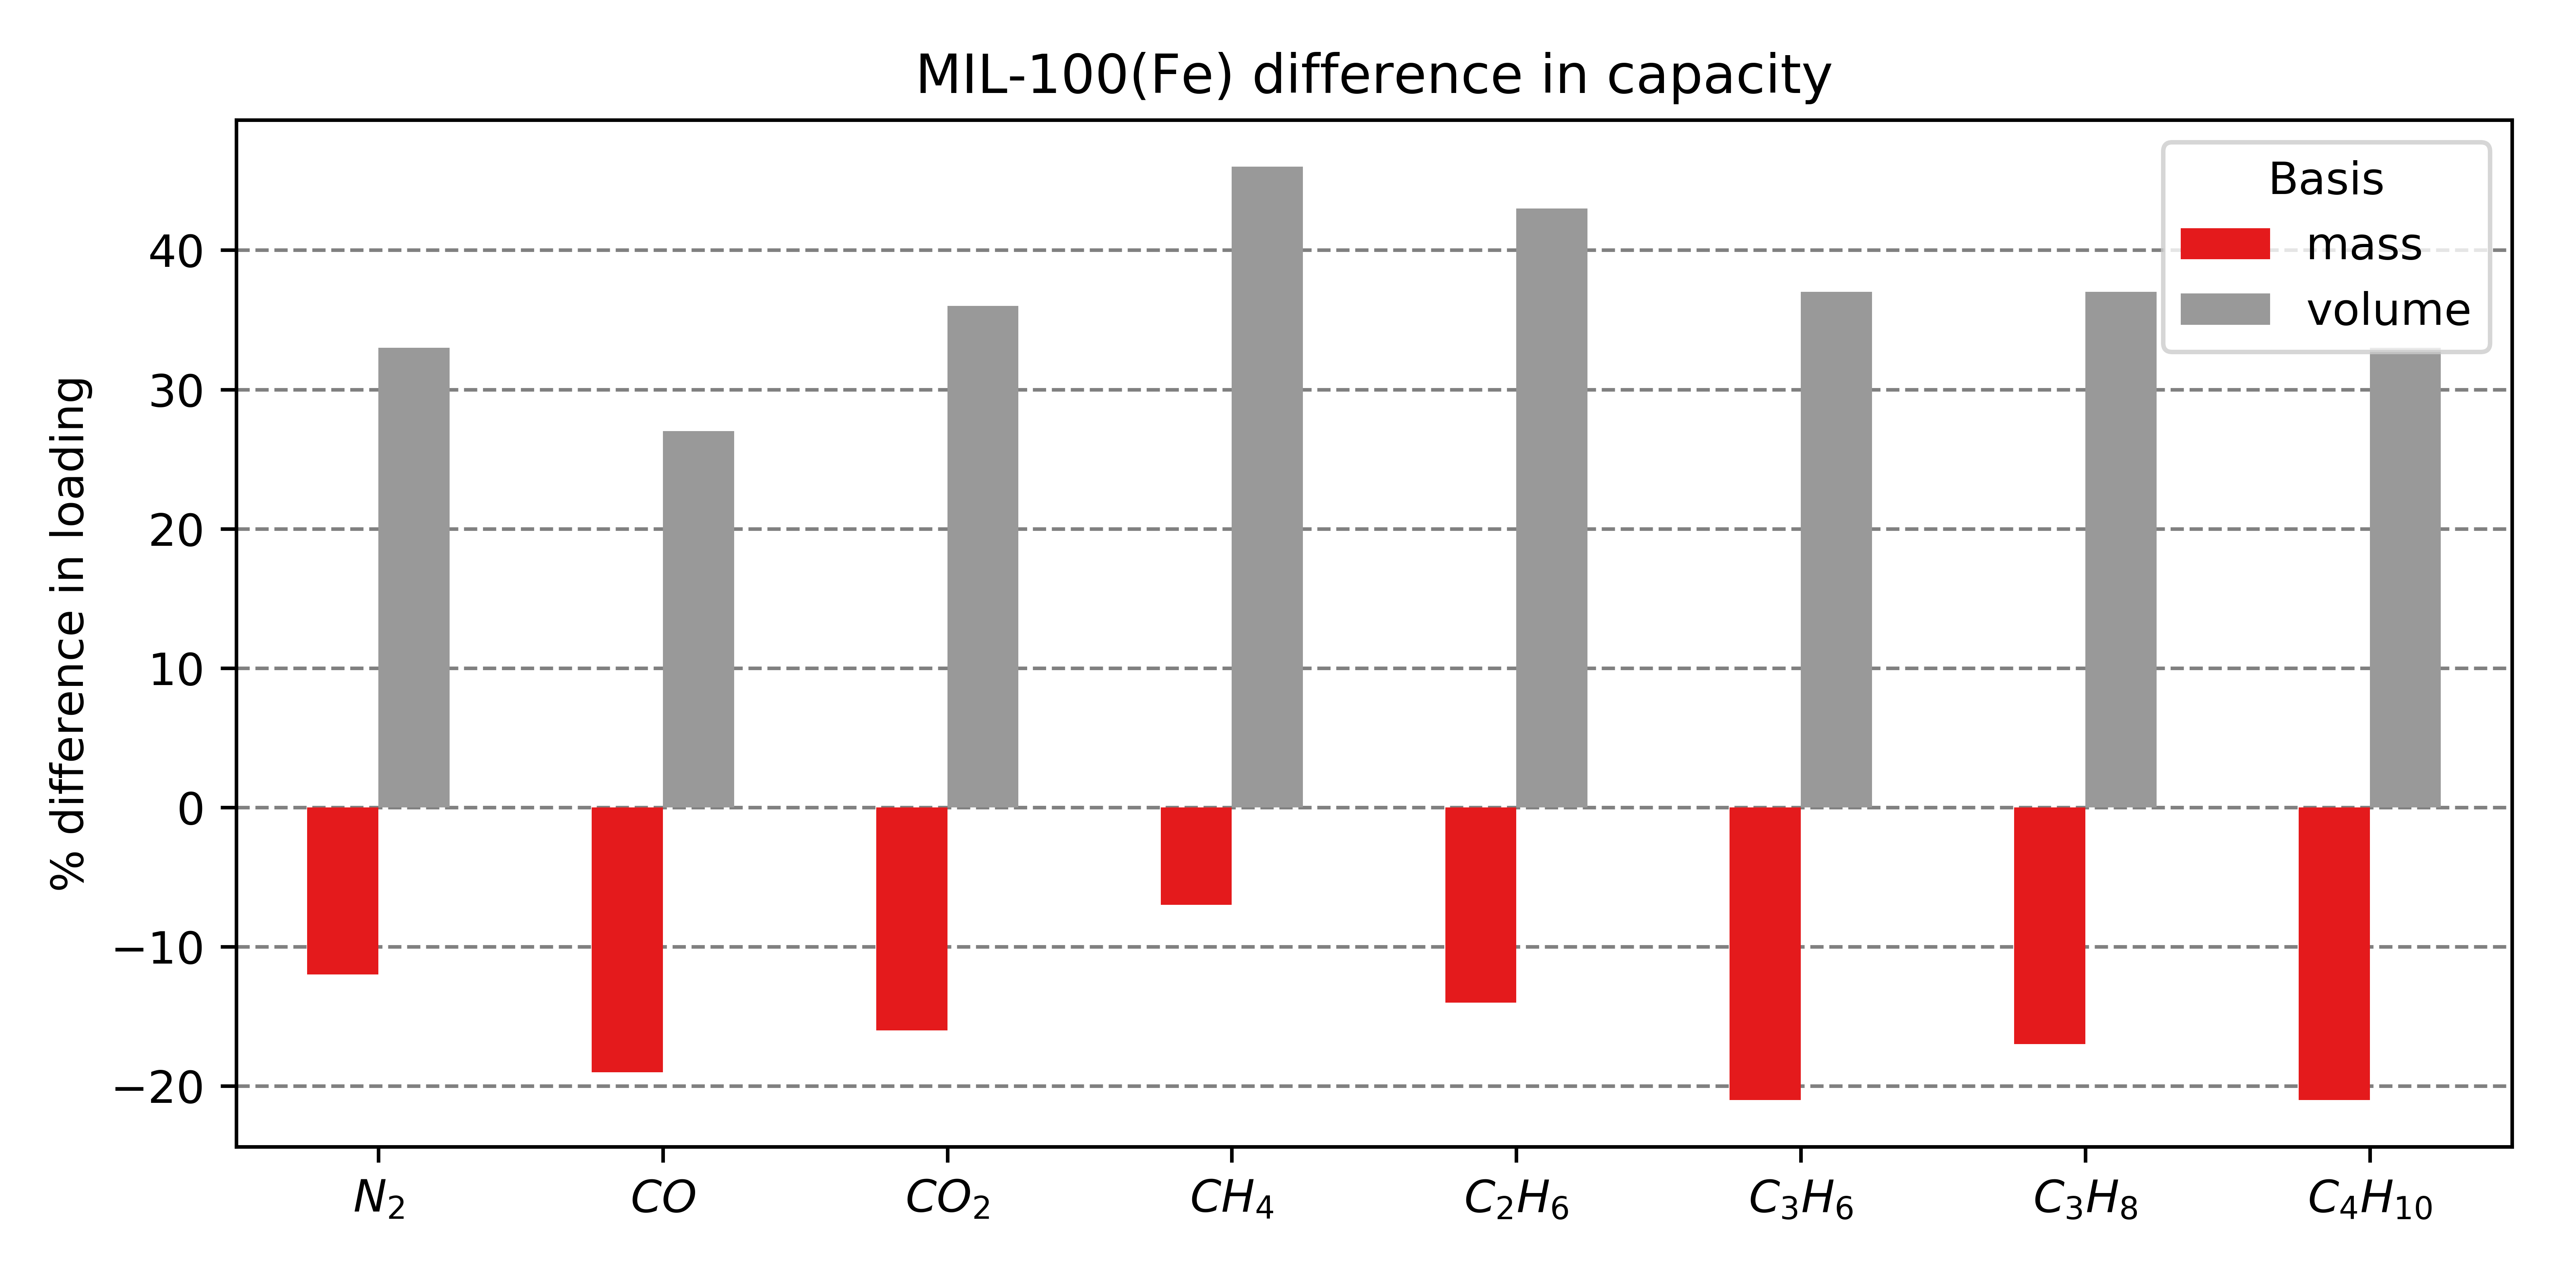
\includegraphics[width=\linewidth]{MIL-100(Fe)-mass-volume}%
		}%
	\end{subfigure}%

	\caption{KPIs extracted from the MIL-100(Fe) adsorption dataset with
		(a) logarithmic initial Henry constant (b) initial enthalpy of
		adsorption and (c) change in adsorption maximum capacity from the powder
		to the alumina shaped version on a mass and volume basis in red and grey
		respectively}%
	\label{shaping:fgr:analysismil100}
\end{figure}